\documentclass[english,floatsintext,man]{apa6}

\usepackage{amssymb,amsmath}
\usepackage{ifxetex,ifluatex}
\usepackage{fixltx2e} % provides \textsubscript
\ifnum 0\ifxetex 1\fi\ifluatex 1\fi=0 % if pdftex
  \usepackage[T1]{fontenc}
  \usepackage[utf8]{inputenc}
\else % if luatex or xelatex
  \ifxetex
    \usepackage{mathspec}
    \usepackage{xltxtra,xunicode}
  \else
    \usepackage{fontspec}
  \fi
  \defaultfontfeatures{Mapping=tex-text,Scale=MatchLowercase}
  \newcommand{\euro}{€}
\fi
% use upquote if available, for straight quotes in verbatim environments
\IfFileExists{upquote.sty}{\usepackage{upquote}}{}
% use microtype if available
\IfFileExists{microtype.sty}{\usepackage{microtype}}{}

% Table formatting
\usepackage{longtable, booktabs}
\usepackage{lscape}
% \usepackage[counterclockwise]{rotating}   % Landscape page setup for large tables
\usepackage{multirow}		% Table styling
\usepackage{tabularx}		% Control Column width
\usepackage[flushleft]{threeparttable}	% Allows for three part tables with a specified notes section
\usepackage{threeparttablex}            % Lets threeparttable work with longtable

% Create new environments so endfloat can handle them
% \newenvironment{ltable}
%   {\begin{landscape}\begin{center}\begin{threeparttable}}
%   {\end{threeparttable}\end{center}\end{landscape}}

\newenvironment{lltable}
  {\begin{landscape}\begin{center}\begin{ThreePartTable}}
  {\end{ThreePartTable}\end{center}\end{landscape}}




% The following enables adjusting longtable caption width to table width
% Solution found at http://golatex.de/longtable-mit-caption-so-breit-wie-die-tabelle-t15767.html
\makeatletter
\newcommand\LastLTentrywidth{1em}
\newlength\longtablewidth
\setlength{\longtablewidth}{1in}
\newcommand\getlongtablewidth{%
 \begingroup
  \ifcsname LT@\roman{LT@tables}\endcsname
  \global\longtablewidth=0pt
  \renewcommand\LT@entry[2]{\global\advance\longtablewidth by ##2\relax\gdef\LastLTentrywidth{##2}}%
  \@nameuse{LT@\roman{LT@tables}}%
  \fi
\endgroup}


  \usepackage{graphicx}
  \makeatletter
  \def\maxwidth{\ifdim\Gin@nat@width>\linewidth\linewidth\else\Gin@nat@width\fi}
  \def\maxheight{\ifdim\Gin@nat@height>\textheight\textheight\else\Gin@nat@height\fi}
  \makeatother
  % Scale images if necessary, so that they will not overflow the page
  % margins by default, and it is still possible to overwrite the defaults
  % using explicit options in \includegraphics[width, height, ...]{}
  \setkeys{Gin}{width=\maxwidth,height=\maxheight,keepaspectratio}
\ifxetex
  \usepackage[setpagesize=false, % page size defined by xetex
              unicode=false, % unicode breaks when used with xetex
              xetex]{hyperref}
\else
  \usepackage[unicode=true]{hyperref}
\fi
\hypersetup{breaklinks=true,
            pdfauthor={},
            pdftitle={Still suspicious: The suspicious coincidence effect revisited},
            colorlinks=true,
            citecolor=blue,
            urlcolor=blue,
            linkcolor=black,
            pdfborder={0 0 0}}
\urlstyle{same}  % don't use monospace font for urls

\setlength{\parindent}{0pt}
%\setlength{\parskip}{0pt plus 0pt minus 0pt}

\setlength{\emergencystretch}{3em}  % prevent overfull lines

\ifxetex
  \usepackage{polyglossia}
  \setmainlanguage{}
\else
  \usepackage[english]{babel}
\fi

% Manuscript styling
\captionsetup{font=singlespacing,justification=justified}
\usepackage{csquotes}
\usepackage{upgreek}



\usepackage{tikz} % Variable definition to generate author note

% fix for \tightlist problem in pandoc 1.14
\providecommand{\tightlist}{%
  \setlength{\itemsep}{0pt}\setlength{\parskip}{0pt}}

% Essential manuscript parts
  \title{Still suspicious: The suspicious coincidence effect revisited}

  \shorttitle{The suspicious coincidence effect revisited}


  \author{Molly L. Lewis\textsuperscript{1,2}~\& Michael C. Frank\textsuperscript{3}}

  \def\affdep{{"", ""}}%
  \def\affcity{{"", ""}}%

  \affiliation{
    \vspace{0.5cm}
          \textsuperscript{1} Computation Institute, University of Chicago\\
          \textsuperscript{2} Department of Psychology, University of Wisconsin, Madison\\
          \textsuperscript{3} Department of Psychology, Stanford University  }

 % If no author_note is defined give only author information if available
      \newcounter{author}
                              \authornote{
            Correspondence concerning this article should be addressed to Molly L. Lewis. E-mail: \href{mailto:mollylewis@uchicago.edu}{\nolinkurl{mollylewis@uchicago.edu}}
          }
                                  
  \note{\(^*\)To whom correspondence should be addressed. E-mail:
\href{mailto:mollylewis@uchicago.edu}{\nolinkurl{mollylewis@uchicago.edu}}}

  \abstract{Enter abstract here. Each new line herein must be indented, like this
line.}
  \keywords{keywords \\

    \indent Word count: X
  }





\usepackage{amsthm}
\newtheorem{theorem}{Theorem}
\newtheorem{lemma}{Lemma}
\theoremstyle{definition}
\newtheorem{definition}{Definition}
\newtheorem{corollary}{Corollary}
\newtheorem{proposition}{Proposition}
\theoremstyle{definition}
\newtheorem{example}{Example}
\theoremstyle{remark}
\newtheorem*{remark}{Remark}
\begin{document}

\maketitle

\setcounter{secnumdepth}{0}



\subsection{Intro}\label{intro}

What is the suspicious coincidence effect?

(Spencer, Perone, Smith, \& Samuelson, 2011; F. Xu \& Tenenbaum, 2007;
Fei Xu \& Tenenbaum, 2007)

Why is it important?

Spencer et al. paper

Methodological differences:

\begin{itemize}
\tightlist
\item
  simultaneous vs.~sequential
\item
  3-1 vs.~1-3
\item
  blocking
\item
  same label vs.~different label
\end{itemize}

other evidence relevant on this replication

Our current paper reports 10 pre-registered experiments. We recover the
suspicious coincidence effect with a large effect size in both
sequential and simultaneous presentation conditions. The effect only
occurs, however, in experiments where the trial with one exemplar is
presented \emph{before} the key trial with three subordinate-consistent
exemplars (the \enquote{suspicious coincidence}). We attribute this
difference to participants' awareness of the possibility of subordinate
generalizations following the three-exemplar trial; in these conditions,
we see a high level of subordinate generalizations even for the
one-exemplar trial (leading to the absence of a difference between
conditions). In sum, and contra SPSS, the \enquote{suspicious
coincidence} effect is robust to sequential presentation. The effect is
sensitive to some features of the general experimental context, however,
suggesting a potential interpretation in terms of the pragmatics of the
task.

\section{Methods}\label{methods}

We report how we determined our sample size, all data exclusions (if
any), all manipulations, and all measures in the study.

\subsection{Participants}\label{participants}

50 participants were recruited on Amazon Mechanical Turk for each of our
10 experiments (N = 500). Participants were paid 40 cents for their
participation

Our sample size was determined based on a pre-registered power
calculation using a meta-anayltic estimate of the effect size from
studies conducted by XT and SPSS (see SI for more details). The chosen
sample size was approximately twice the estimated sample size necessary
to obtain a power of 1.

\begin{itemize}
\tightlist
\item
  Exclusions?
\end{itemize}

\subsection{Stimuli}\label{stimuli}

Our stimuli closely resembled that of XT and SPSS. The pictures
consisted of three sets of 15 photos from different basic level
categories (vegetables, vehicles and animals). Within each category,
five were subordinate exemplars (e.g.~green pepper), four were basic
level exemplars (e.g.~peppers), and six were superordinate exemplars
(e.g.~vegetables). The exemplars were divided into a learning and test
set.

Novel labels

\subsection{Procedure}\label{procedure}

\subsubsection{Manipulations:}\label{manipulations}

\begin{enumerate}
\def\labelenumi{(\arabic{enumi})}
\tightlist
\item
  Timing
\item
  Order
\item
  Blocking
\item
  Labels
\end{enumerate}

\subsection{Data analysis}\label{data-analysis}

We used R (3.4.1, R Core Team, 2017) and the R-packages \emph{bindrcpp}
(0.2, Müller, 2017), \emph{broom} (0.4.2, Robinson, 2017),
\emph{compute.es} (0.2.4, Re, 2013), \emph{dplyr} (0.7.2, Wickham,
Francois, Henry, \& Müller, 2017), \emph{forcats} (0.2.0, Wickham,
2017a), \emph{ggplot2} (2.2.1, Wickham, 2009), \emph{jsonlite} (1.5,
Ooms, 2014), \emph{kableExtra} (0.4.0, Zhu, 2017), \emph{knitr} (1.17,
Xie, 2015), \emph{langcog} (0.1.9001, Braginsky, Yurovsky, \& Frank,
n.d.), \emph{Matrix} (1.2.10, Bates \& Maechler, 2017), \emph{metafor}
(2.0.0, Viechtbauer, 2010), \emph{papaja} (0.1.0.9492, Aust \& Barth,
2017), \emph{png} (0.1.7, Urbanek, 2013), \emph{purrr} (0.2.3, Henry \&
Wickham, 2017), \emph{readr} (1.1.1, Wickham, Hester, \& Francois,
2017), \emph{rmarkdown} (1.6, Allaire et al., 2017), \emph{stringr}
(1.2.0, Wickham, 2017b), \emph{tibble} (1.3.3, Müller \& Wickham, 2017),
\emph{tidyr} (0.6.3, Wickham, 2017c), and \emph{tidyverse} (1.1.1,
Wickham, 2017d) for all our analyses.

\section{Results}\label{results}

\begin{figure}
\centering
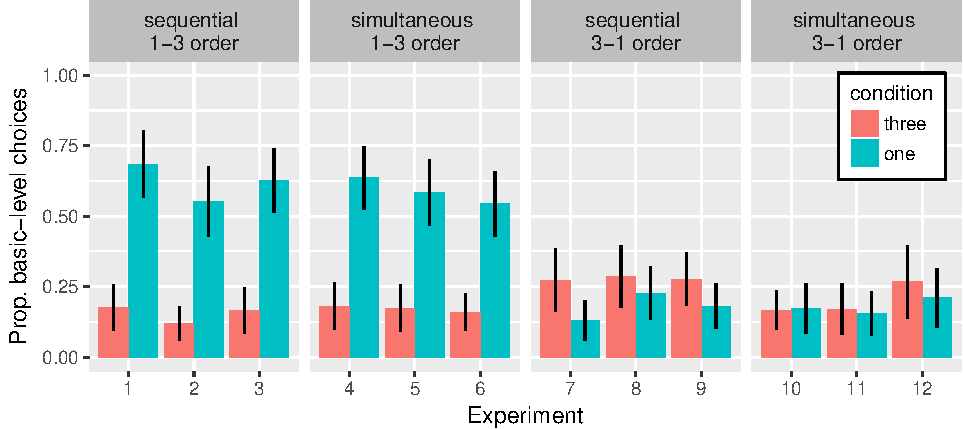
\includegraphics{xtmem_files/figure-latex/unnamed-chunk-2-1.pdf}
\caption{\label{fig:unnamed-chunk-2}Mean proportion generalization to basic
level exemplars in the one (green) and three (pink) subordinate exemplar
conditions for all 10 of our experiments. Each facet corresponds to a
pairing of presentation timing (sequential vs.~simultaneous) and trial
order (1-3 vs.~3-1). Error bars are bootstrapped 95\% confidence
intervals.}
\end{figure}

\begin{table}

\caption{\label{tab:unnamed-chunk-3}Summary of our 10 experiments.}
\centering
\fontsize{12}{14}\selectfont
\begin{tabular}[t]{crrrrrrr}
\toprule
\multicolumn{2}{c}{ } & \multicolumn{4}{c}{Manipulations} & \multicolumn{1}{c}{ } \\
\cmidrule(l{2pt}r{2pt}){3-6}
Exp. & N & Timing & Order & Blocking & Label & Effect Size & Original 
Exp.\\
\midrule
1 & 50 & seq. & 1-3 & random & same & 1.42 [1.32, 1.52] & \\
2 & 50 & seq. & 1-3 & random & diff. & 1.26 [1.18, 1.34] & \\
3 & 50 & simult. & 1-3 & random & same & 1.32 [1.24, 1.4] & XT E1/E2\\
4 & 50 & simult. & 1-3 & random & same & 1.14 [1.06, 1.22] & XT E1/E2\\
5 & 50 & simult. & 1-3 & random & diff. & 1.16 [1.08, 1.24] & \\
\addlinespace
6 & 50 & seq. & 3-1 & blocked & diff. & -0.44 [-0.52, -0.36] & SPSS E2/E3\\
7 & 50 & seq. & 3-1 & blocked & same & -0.17 [-0.25, -0.09] & \\
8 & 50 & simult. & 3-1 & blocked & diff. & 0.02 [-0.06, 0.1] & SPSS ES1/ES2\\
9 & 50 & simult. & 3-1 & blocked & diff. & -0.06 [-0.14, 0.02] & \\
10 & 50 & simult. & 3-1 & blocked & same & -0.14 [-0.22, -0.06] & \\
\bottomrule
\multicolumn{8}{l}{\textsuperscript{1} N = sample size; Timing = presentation timing (sequential or simultaneous); Order =}\\
\multicolumn{8}{l}{relative ordering of 1 and 3 subordinate trials; Blocking = trials blocked by category or}\\
\multicolumn{8}{l}{pseudorandom; Label = same or different label in 1 and 3 trials; Effect size = Cohen's d}\\
\multicolumn{8}{l}{[95\% CI]; Orginal Exp. = corresponding prior experiment.}\\
\end{tabular}
\end{table}

\begin{figure}
\centering
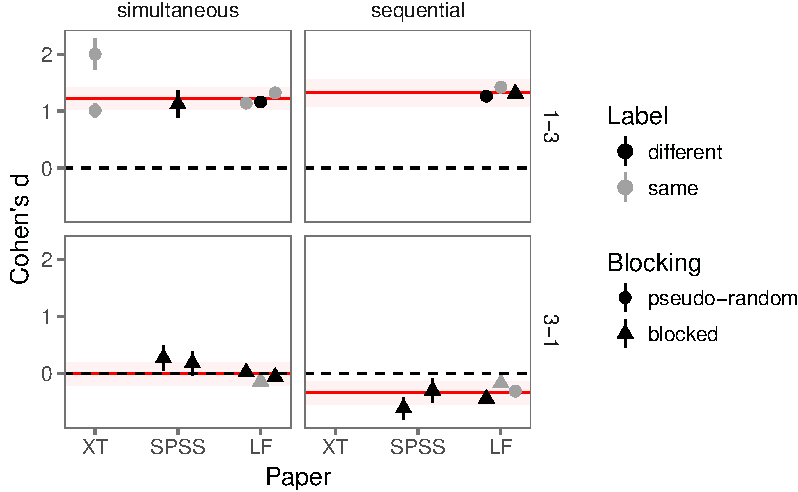
\includegraphics{xtmem_files/figure-latex/unnamed-chunk-4-1.pdf}
\caption{\label{fig:unnamed-chunk-4}Cumulative plot of effect sizes for all
17 studies conducted on the suspicious coincidence effect by XT (Xu \&
Tenenbaum, 2007a), SPSS (Spencer, et al, 2011), and the current authors.
Facets along the vertical indicate whether the single exemplar trial
occurred first (1-3) or second (3-1). Facets along the horizontal
indicate whether the exemplars were presented simulateously as in XT or
sequentially as in SPSS. Point color indicates whether the single
exemplar and three subordinate exemplars received the same (grey) or
different (black) label. Point shape indicates whether trials were
blocked by category (circle) or pseudo-random (triangle). Points are
jittered along the x-axis for visibility. The red line reflects the
meta-analytic estimate of the effect size. All error bars are 95\%
confidence intervals.}
\end{figure}

\begin{table}

\caption{\label{tab:unnamed-chunk-5}Meta-analytic model with manipulations as fixed effects.}
\centering
\fontsize{12}{14}\selectfont
\begin{tabular}[t]{lrrr}
\toprule
Fixed effect & beta & z-value & p-value\\
\midrule
Intercept & 1.12 [0.44, 1.8] & 3.23 & <.0001\\
Simultaneous vs. sequential timing & -0.15 [-0.38, 0.09] & -1.24 & 0.22\\
1-3 vs. 3-1 condition order & -1.22 [-1.92, -0.51] & -3.36 & <.0001\\
Different vs. same label & 0.02 [-0.22, 0.26] & 0.19 & 0.85\\
Blocked vs. random trial order & 0.17 [-0.55, 0.89] & 0.47 & 0.64\\
\bottomrule
\end{tabular}
\end{table}

\section{Discussion}\label{discussion}

\newpage

\section{References}\label{references}

\setlength{\parindent}{-0.5in} \setlength{\leftskip}{0.5in}

\hypertarget{refs}{}
\hypertarget{ref-R-rmarkdown}{}
Allaire, J., Cheng, J., Xie, Y., McPherson, J., Chang, W., Allen, J.,
\ldots{} Arslan, R. (2017). \emph{Rmarkdown: Dynamic documents for r}.
Retrieved from \url{https://CRAN.R-project.org/package=rmarkdown}

\hypertarget{ref-R-papaja}{}
Aust, F., \& Barth, M. (2017). \emph{papaja: Create APA manuscripts with
R Markdown}. Retrieved from \url{https://github.com/crsh/papaja}

\hypertarget{ref-R-Matrix}{}
Bates, D., \& Maechler, M. (2017). \emph{Matrix: Sparse and dense matrix
classes and methods}. Retrieved from
\url{https://CRAN.R-project.org/package=Matrix}

\hypertarget{ref-R-langcog}{}
Braginsky, M., Yurovsky, D., \& Frank, M. (n.d.). \emph{Langcog:
Language and cognition lab things}. Retrieved from
\url{http://github.com/langcog/langcog}

\hypertarget{ref-R-purrr}{}
Henry, L., \& Wickham, H. (2017). \emph{Purrr: Functional programming
tools}. Retrieved from \url{https://CRAN.R-project.org/package=purrr}

\hypertarget{ref-R-bindrcpp}{}
Müller, K. (2017). \emph{Bindrcpp: An 'rcpp' interface to active
bindings}. Retrieved from
\url{https://CRAN.R-project.org/package=bindrcpp}

\hypertarget{ref-R-tibble}{}
Müller, K., \& Wickham, H. (2017). \emph{Tibble: Simple data frames}.
Retrieved from \url{https://CRAN.R-project.org/package=tibble}

\hypertarget{ref-R-jsonlite}{}
Ooms, J. (2014). The jsonlite package: A practical and consistent
mapping between json data and r objects. \emph{arXiv:1403.2805
{[}Stat.CO{]}}. Retrieved from \url{https://arxiv.org/abs/1403.2805}

\hypertarget{ref-R-base}{}
R Core Team. (2017). \emph{R: A language and environment for statistical
computing}. Vienna, Austria: R Foundation for Statistical Computing.
Retrieved from \url{https://www.R-project.org/}

\hypertarget{ref-R-compute.es}{}
Re, A. C. D. (2013). \emph{Compute.es: Compute effect sizes}. \emph{R
Package}. Retrieved from
\url{http://cran.r-project.org/web/packages/compute.es}

\hypertarget{ref-R-broom}{}
Robinson, D. (2017). \emph{Broom: Convert statistical analysis objects
into tidy data frames}. Retrieved from
\url{https://CRAN.R-project.org/package=broom}

\hypertarget{ref-spencer2011learning}{}
Spencer, J. P., Perone, S., Smith, L. B., \& Samuelson, L. K. (2011).
Learning words in space and time: Probing the mechanisms behind the
suspicious-coincidence effect. \emph{Psychological Science},
\emph{22}(8), 1049--1057.

\hypertarget{ref-R-png}{}
Urbanek, S. (2013). \emph{Png: Read and write png images}. Retrieved
from \url{https://CRAN.R-project.org/package=png}

\hypertarget{ref-R-metafor}{}
Viechtbauer, W. (2010). Conducting meta-analyses in R with the metafor
package. \emph{Journal of Statistical Software}, \emph{36}(3), 1--48.
Retrieved from \url{http://www.jstatsoft.org/v36/i03/}

\hypertarget{ref-R-ggplot2}{}
Wickham, H. (2009). \emph{Ggplot2: Elegant graphics for data analysis}.
Springer-Verlag New York. Retrieved from \url{http://ggplot2.org}

\hypertarget{ref-R-forcats}{}
Wickham, H. (2017a). \emph{Forcats: Tools for working with categorical
variables (factors)}. Retrieved from
\url{https://CRAN.R-project.org/package=forcats}

\hypertarget{ref-R-stringr}{}
Wickham, H. (2017b). \emph{Stringr: Simple, consistent wrappers for
common string operations}. Retrieved from
\url{https://CRAN.R-project.org/package=stringr}

\hypertarget{ref-R-tidyr}{}
Wickham, H. (2017c). \emph{Tidyr: Easily tidy data with 'spread()' and
'gather()' functions}. Retrieved from
\url{https://CRAN.R-project.org/package=tidyr}

\hypertarget{ref-R-tidyverse}{}
Wickham, H. (2017d). \emph{Tidyverse: Easily install and load
'tidyverse' packages}. Retrieved from
\url{https://CRAN.R-project.org/package=tidyverse}

\hypertarget{ref-R-dplyr}{}
Wickham, H., Francois, R., Henry, L., \& Müller, K. (2017). \emph{Dplyr:
A grammar of data manipulation}. Retrieved from
\url{https://CRAN.R-project.org/package=dplyr}

\hypertarget{ref-R-readr}{}
Wickham, H., Hester, J., \& Francois, R. (2017). \emph{Readr: Read
rectangular text data}. Retrieved from
\url{https://CRAN.R-project.org/package=readr}

\hypertarget{ref-R-knitr}{}
Xie, Y. (2015). \emph{Dynamic documents with R and knitr} (2nd ed.).
Boca Raton, Florida: Chapman; Hall/CRC. Retrieved from
\url{https://yihui.name/knitr/}

\hypertarget{ref-xu2007word}{}
Xu, F., \& Tenenbaum, J. (2007). Word learning as Bayesian inference.
\emph{Psychological Review}, \emph{114}(2), 245.

\hypertarget{ref-xu2007}{}
Xu, F., \& Tenenbaum, J. B. (2007). Sensitivity to sampling in Bayesian
word learning. \emph{Developmental Science}, \emph{10}(3), 288--297.

\hypertarget{ref-R-kableExtra}{}
Zhu, H. (2017). \emph{KableExtra: Construct complex table with 'kable'
and pipe syntax}. Retrieved from
\url{https://CRAN.R-project.org/package=kableExtra}






\end{document}
